\chapter{Design Proposal}
\label{ch:design-proposal}

\section{Generic CubeSat Structure}
% Input below the existing Generic CubeSat Structure section heading.
% The 18-paper count includes four RAX/enterprise predecessors and fourteen
% CRM/CSRM development or companion-method papers. It excludes application
% studies, specifications, and separately cited Space Symposium venue versions.
\label{section:generic-cubesat-structure}

The CubeSat System Reference Model (CSRM) is a reusable SysML model of a CubeSat mission's logical space and ground architecture. It links stakeholders, requirements, behaviors, technical measures and architecture to support the development of mission-specific models \citep{kaslow2020csrm}. The surveyed literature identifies 18 papers in its core research lineage, covering the Radio Aurora Explorer predecessors, reference model development, and companion methods for behavior, technical measurement, validation and mission engineering \citep{review-1646,review-1621,review-1554,review-1563,review-1494,review-1487,review-1451,review-1446,kaslow2017status3,kaslow2017behaviors,kaslow2018verification,review-1288,kaslow2018status4,kaslow2019csrm,kaslow2020csrm,review-1051,kaslow2022mission,rudder2026metamodel}. The International Council on Systems Engineering (INCOSE) Space Systems Working Group began investigating CubeSat modeling in 2011. Work progressed from mission demonstrations to a generic reference model and its validation, then to Object Management Group (OMG) specifications: CSRM 1.0 in 2023 and CSRM 1.1 in 2025 \citep{review-1494,kaslow2019csrm,omg2023csrm,omg2025csrm}. Applications include student CubeSat design through the Parkinson Sat 1U (PSAT1U) template, EPS conceptual design and concurrent engineering tutorials \citep{review-1112,review-1009,deutsch2022comet}. Its applicability to cislunar missions has also been assessed \citep{review-0699}.

The framework will use this reference structure as the starting point for its SysML v2 CubeSat model. Figures~\ref{fig:csrm-mission-structure}--\ref{fig:csrm-eps-components} show the mission structure, the nine CubeSat subsystems and the six EPS component groups. Mission teams will tailor these logical categories to their missions. Reference part multiplicities describe the template. Detailed design will establish physical quantities, electrical connections and implementation choices.
The CSRM EPS model will be tailored to each mission by selecting a topology alternative using the variation points defined by El Hachimi et al. \citep[Fig.~1, Sec.~4]{handpicked-0003}. Figure~\ref{fig:csrm-eps-topology} maps the relevant CSRM component groups to those choices.

% These authored views use the translated architecture from the 18 November
% 2025 CSRM model. The complete profile, behaviors and traceability are outside
% the current translation. The diagrams establish no SysML v2 conformance or
% runtime validation. The orbit reference is a chosen translation feature.

\begin{landscape}
\captionsetup{font=small,skip=4pt}
\begin{figure}[p]
\centering
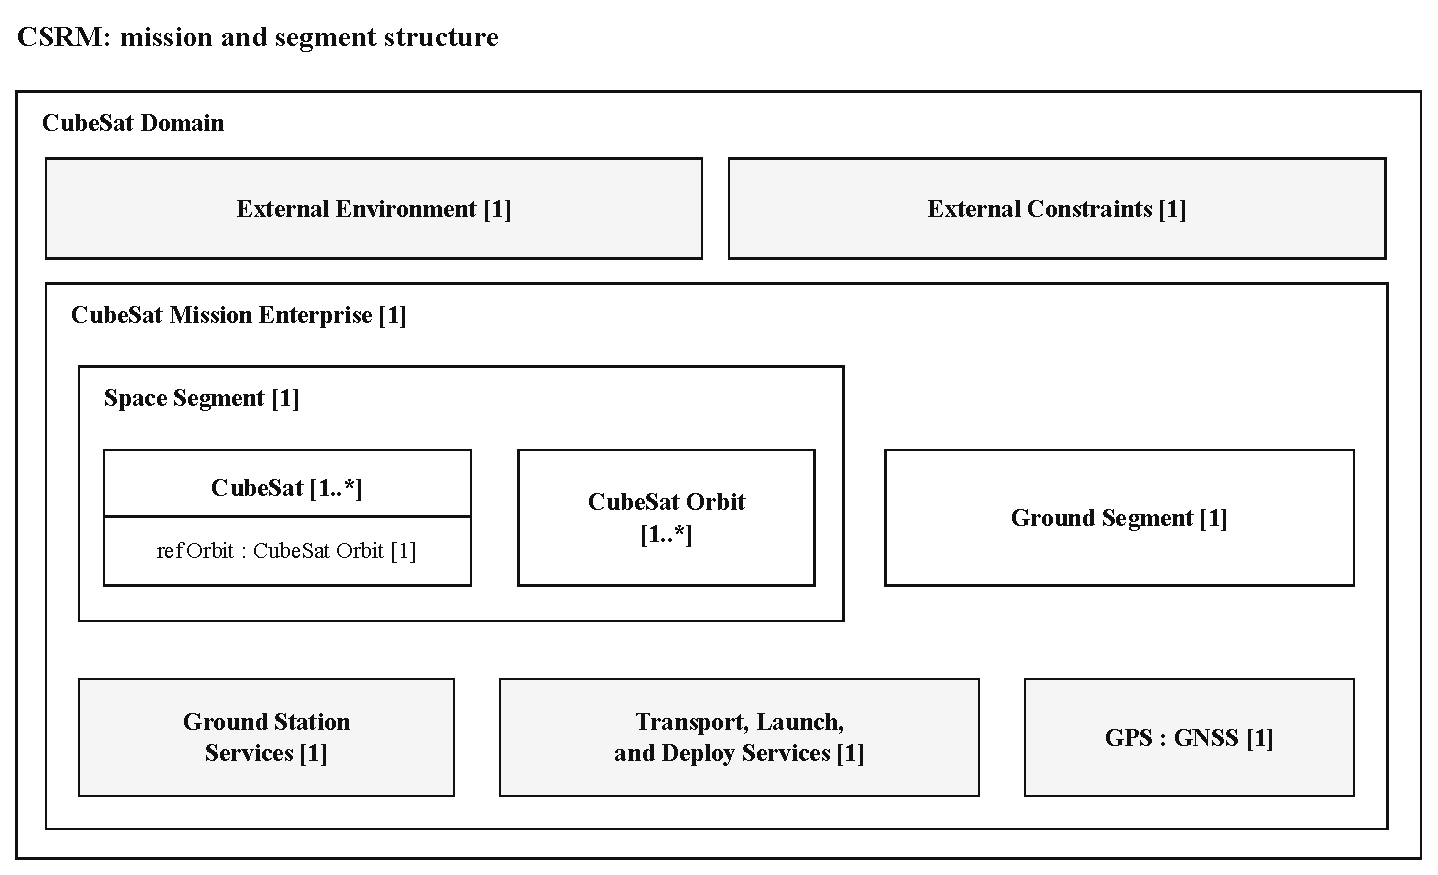
\includegraphics[width=\linewidth,height=\dimexpr\textheight-95pt\relax,keepaspectratio]{fig/csrm-mission-structure.pdf}
\caption[CSRM mission and segment structure.]{CSRM mission and segment structure. Nested rectangles denote composition. Brackets give part multiplicities. Light gray identifies external context and services. Orbits are modeled elements of the Space Segment. Each CubeSat has an orbit reference, with no individual spacecraft-to-orbit pairing specified in this view. Adapted from the CSRM reference model, copyright 2022 INCOSE Space Systems Working Group and OMG Space Domain Task Force, \href{https://creativecommons.org/licenses/by/4.0/}{CC BY 4.0} \citep{incose2025csrmmodel}.}
\label{fig:csrm-mission-structure}
\end{figure}
\clearpage

\begin{figure}[p]
\centering
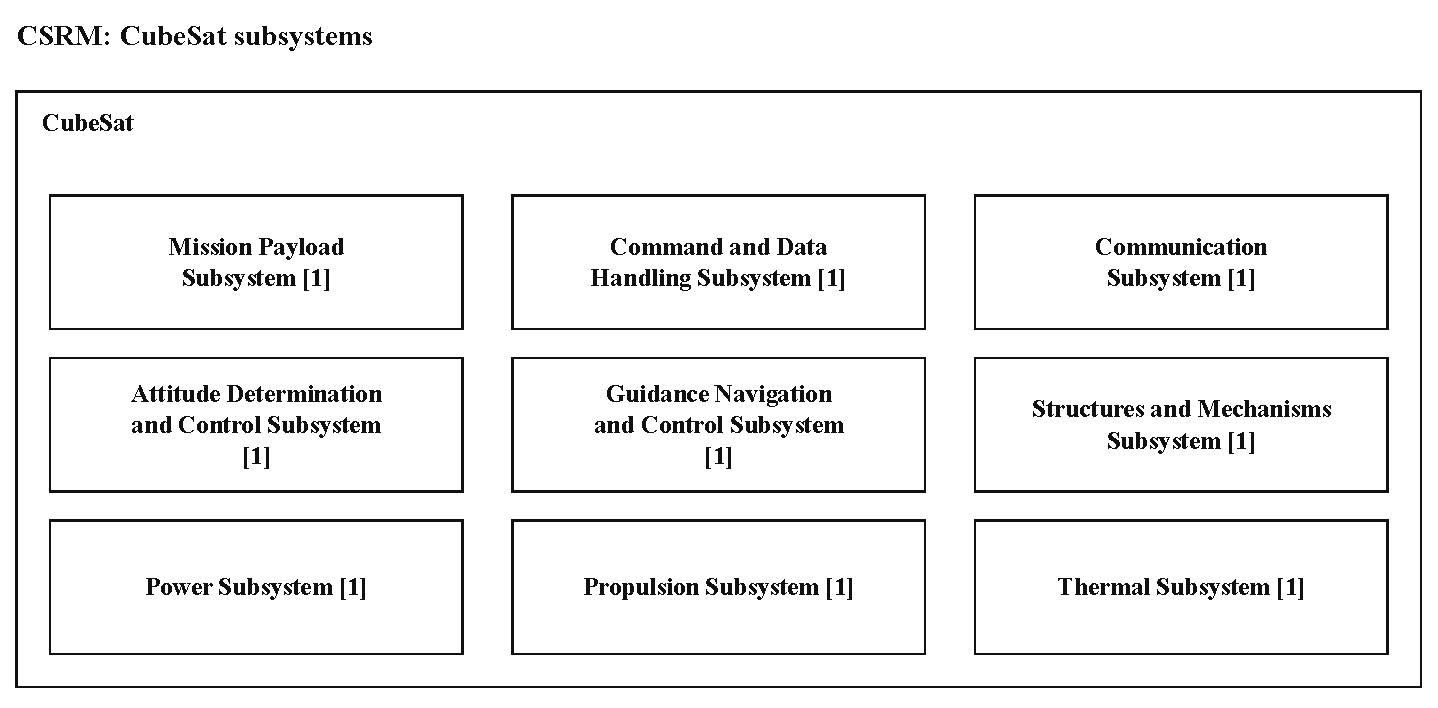
\includegraphics[width=\linewidth,height=\dimexpr\textheight-80pt\relax,keepaspectratio]{fig/csrm-cubesat-subsystems.pdf}
\caption[CSRM CubeSat subsystems.]{CSRM CubeSat subsystems. The reference architecture contains one part for each of nine subsystem categories. Power Subsystem is the EPS. Mission-specific models can omit, combine or refine categories to meet mission needs \citep{kaslow2020csrm}. The view shows logical composition. It specifies no subsystem interfaces or allocation to circuit boards. Adapted from the CSRM reference model \citep{incose2025csrmmodel}.}
\label{fig:csrm-cubesat-subsystems}
\end{figure}
\clearpage

\begin{figure}[p]
\centering
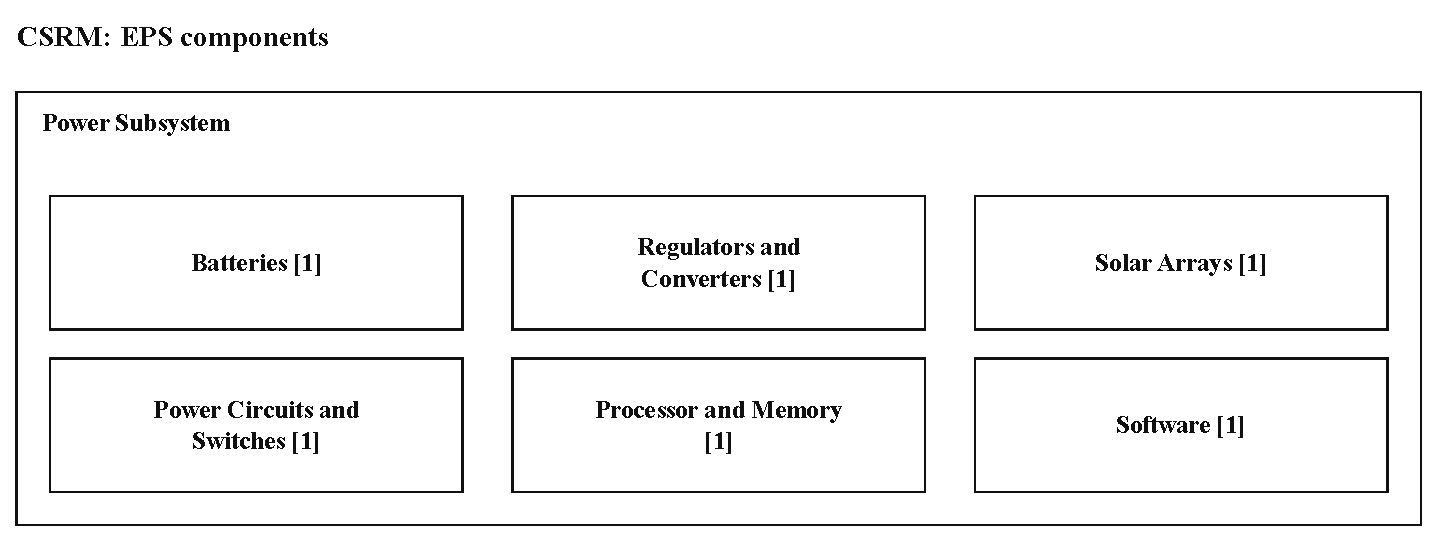
\includegraphics[width=\linewidth,height=\dimexpr\textheight-80pt\relax,keepaspectratio]{fig/csrm-eps-components.pdf}
\caption[CSRM EPS component groups.]{CSRM EPS component groups. The Power Subsystem contains six reference component categories, including processing and software. Batteries and Solar Arrays each denote an aggregate category. Multiplicity [1] identifies one reference part per category. Detailed design will define the numbers of cells, panels, converters and switches, together with their electrical connections. Adapted from the CSRM reference model \citep{incose2025csrmmodel}.}
\label{fig:csrm-eps-components}
\end{figure}
\clearpage
\begin{figure}[p]
\centering
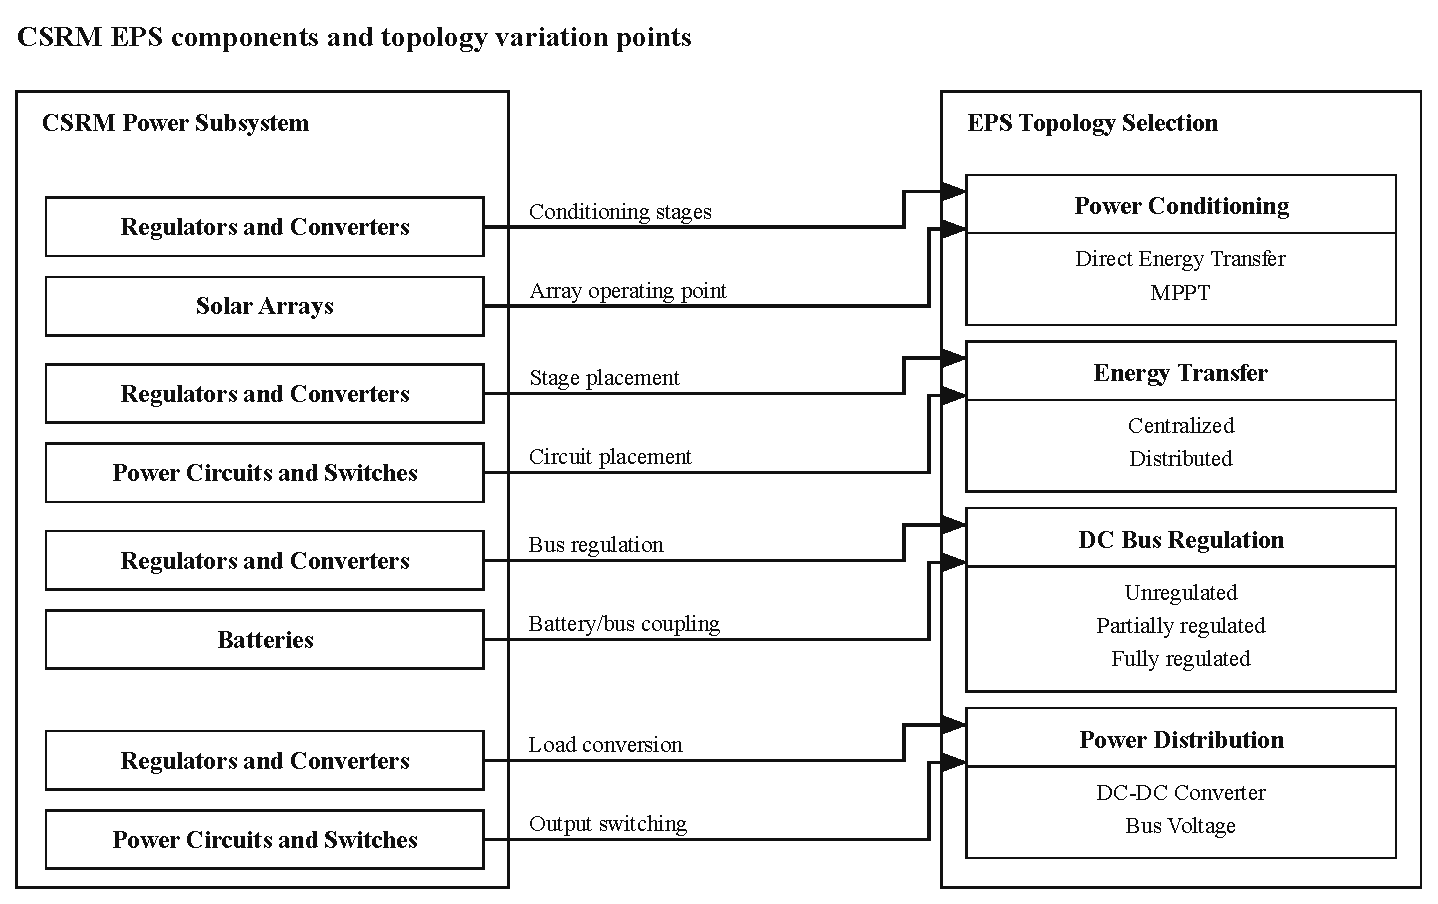
\includegraphics[width=\linewidth,height=\dimexpr\textheight-95pt\relax,keepaspectratio]{fig/csrm-eps-topology.pdf}
\caption[CSRM EPS components and topology variation points.]{CSRM EPS components and topology variation points. Arrows express design associations proposed for this framework. Route labels identify the affected design roles. Repeated component names denote the same CSRM groups \citep{incose2025csrmmodel}. The alternatives follow El Hachimi et al. \citep[Fig.~1, Sec.~4]{handpicked-0003}. The view focuses on hardware topology. Processing and software remain in the reference structure shown in Figure~\ref{fig:csrm-eps-components}. No topology alternative is selected in this view.}
\label{fig:csrm-eps-topology}
\end{figure}
\clearpage
\end{landscape}


\section{Orbit Requirements and Power Budget}

\subsection{Mission analogues from operational descriptions}

When orbit information is unavailable, the framework will accept a plain text concept of operations. It will encode that text and revisioned descriptions of existing missions as semantic embeddings (numerical text vectors), then rank analogues by cosine similarity. Each result will identify the exact mission, source revision and parameter epoch. It will present sourced altitude values or ranges, orbit context and missing fields, while distinguishing flown conditions from intended or study assumptions. Similarity will provide retrieval ranks rather than suitability probabilities. An engineer will review alternatives and explicitly accept each parameter transferred into the mission model. Acceptance will create a mission revision and invalidate dependent results through the normal dependency process. Independent analysis will assess launch opportunities, coverage, revisit, resolution, illumination and orbital constraints. A mission description will establish no unique orbit or validation of its feasibility.

\subsection{Preliminary EPS sizing}

Preliminary EPS sizing will follow El Hachimi et al. \citep[Secs.~2--3, Eqs.~(1)--(10)]{handpicked-0003}.

With altitude $h$ in km, Earth radius $R_e=6378~\mathrm{km}$ and gravitational parameter $\mu=398601~\mathrm{km^3/s^2}$, the orbit, sunlight and eclipse periods (s) are:
\begin{align}
    T_o &= 2\pi\sqrt{\frac{(R_e+h)^3}{\mu}},
    \label{eq:orbit-period} \\
    T_s &= \left(\frac{1}{2}+\frac{\psi}{\pi}\right)T_o,
    \label{eq:sunlight-period} \\
    T_e &= \left(\frac{1}{2}-\frac{\psi}{\pi}\right)T_o,
    \label{eq:eclipse-period} \\
    \psi &= \arccos\left(\frac{R_e}{R_e+h}\right).
    \label{eq:eclipse-geometry}
\end{align}

Subsystem powers and duty cycles give the sunlight and eclipse energies $E_s$ and $E_e$. With corresponding energy path efficiencies $X_s$ and $X_e$, the minimum solar panel power is:
\begin{equation}
    P_{\mathrm{sp}_{\min}} = \frac{\frac{E_s}{X_s}+\frac{E_e}{X_e}}{T_s}.
    \label{eq:minimum-panel-power}
\end{equation}

Solar cell power at end of life (subscript EOL) uses maximum power point voltage $V_{\mathrm{mp}_{\mathrm{EOL}}}$ and current $I_{\mathrm{mp}_{\mathrm{EOL}}}$. The required cell count is $N_{\mathrm{sc}}$:
\begin{align}
    P_{\mathrm{sc}_{\mathrm{EOL}}} &= V_{\mathrm{mp}_{\mathrm{EOL}}} I_{\mathrm{mp}_{\mathrm{EOL}}},
    \label{eq:solar-cell-eol-power} \\
    N_{\mathrm{sc}} &= \frac{P_{\mathrm{sp}_{\min}}}{P_{\mathrm{sc}_{\mathrm{EOL}}}}.
    \label{eq:solar-cell-count}
\end{align}

For mission lifetime $N_{\mathrm{lifetime}}$ in years, $N_{\mathrm{day/year}}$ days per year and $N_{\mathrm{orbit/day}}$ orbits per day, the required cycle count sets the depth of discharge limit $\mathrm{DoD}$. Battery energy includes degradation margin $M$:
\begin{align}
    N_{\mathrm{cycle}} &= N_{\mathrm{lifetime}}\cdot N_{\mathrm{day/year}}\cdot N_{\mathrm{orbit/day}},
    \label{eq:battery-mission-cycles} \\
    N_{\mathrm{cycle}} &= a\cdot \mathrm{DoD}^{b},
    \label{eq:battery-cycle-life} \\
    E_{\mathrm{Battery}} &= \frac{E_e}{\mathrm{DoD}}(1+M).
    \label{eq:battery-energy}
\end{align}

\section{EPS Components and Loads Generic Models}
\label{section:eps-generic-models}

The framework will define reusable models for the six CSRM EPS component groups and for the loads they supply. These models will provide the schema for browsing COTS products and assembling candidate EPS configurations. A catalog entry will describe a particular product and revision. A part usage in a candidate architecture will reference that entry and specify its quantity, supported configuration, installation and connections. One integrated EPS board can implement several CSRM groups. Logical role allocations will reference the same physical usage. Its physical properties will be accounted for once.

\paragraph{Common characterization.}
Luccisano et al. contribute shared component identity, manufacturer, mass, power by operating mode and margins. Their distinction between aggregate and detailed component budgets supports explicit accounting boundaries \citep[Secs.~3.1--3.2]{luccisano2024formalization}. Ceglarek and Bertrand contribute a catalog built from manufacturer datasheets with controlled parameter meanings and units. Their experience with inconsistent datasheets motivates retaining the original value and its reviewed interpretation \citep[Sec.~3]{review-0257}. The proposed schema will extend these contributions with source revisions, operating conditions, uncertainty, supported configurations and interface descriptions. These extensions will make catalog comparisons assessable.

\paragraph{Solar arrays and batteries.}
El Hachimi et al. supply the solar maximum power point and EOL properties, battery energy and cycle-life criteria, and examples of named cells and their arrangements \citep[Secs.~3 and~6.2]{handpicked-0003}. Casado et al. contribute solar current--voltage curves with irradiance and temperature conditions, battery discharge curves and internal resistance \citep[Secs.~2.1 and~2.3]{review-0573}. Boan contributes the series/parallel configuration and mission illumination needed to assess a selected assembly \citep[Sec.~3]{review-0289}. These sources motivate separate cell and assembly records, conditional electrical characteristics and installation geometry. Wijaya et al. contribute fixed commercial product properties alongside sized alternatives. Purchased panels and packs will retain their specified dimensions, mass and ratings \citep[Sec.~III.A--B, Appendix]{review-0145}.

\paragraph{Regulators, converters, power circuits and switches.}
El Hachimi et al. contribute conditioning and bus alternatives, converter input compatibility, independently controlled outputs, protection thresholds, timing and autonomous protection functions \citep[Secs.~4 and~7.1--7.6]{handpicked-0003}. Casado et al. contribute regulator operating modes and transitions, protected output rails, and distribution efficiency estimates based on measurements \citep[Secs.~2.2 and~2.4]{review-0573}. The models will therefore distinguish conversion capabilities, electrical operating limits, loss data, channel organization and protection behavior. A controller integrated circuit record will retain its required external circuit. Its ratings alone will establish no complete converter or protected output.

\paragraph{Processor, memory and software.}
El Hachimi et al. contribute the EPS processor and memory roles, telemetry, output control and hardware/software protection responsibilities \citep[Secs.~7.2--7.5]{handpicked-0003}. Halvorson and Thomas distinguish architecture and interface definitions from implemented behavior and software build dependencies \citep[Secs.~3--4]{review-0853}. The framework will extend these contributions with host compatibility, memory requirements, task timing and versioned service definitions. Software will reference its execution host. Its execution power and physical mass will be included in that host's accounting boundary.

\paragraph{Loads.}
Luccisano et al. contribute power states and their allocation to operating modes \citep[Secs.~3.1--3.2]{luccisano2024formalization}. Casado et al. contribute electrical load profiles and their supply through regulated and unregulated lines \citep[Sec.~2.4]{review-0573}. El Hachimi et al. add maximum-load and protection cases \citep[Secs.~7.4--7.5 and~8.1.4]{handpicked-0003}. The generic load model will combine mode consumption, voltage tolerance, startup pulses, scheduling and shedding constraints. The same description will apply to spacecraft loads and to EPS consumers such as processors and battery heaters.

Figure~\ref{fig:eps-component-models} summarizes the proposed definitions. SysML v2 part definitions will describe hardware and software categories. Attribute definitions will describe structured specifications and physical quantities. Port definitions will describe connection points, and interface definitions will constrain compatible connections \citep[Secs.~7.7, 7.11--7.14 and~9.8]{omg2026sysml2}. Directed command and telemetry items will use requester/provider port conjugation. Physical electrical interfaces will use across voltage and through current quantities with a declared sign convention. Tables~\ref{tab:eps-catalog-records}--\ref{tab:eps-specialized-properties} define the schema summarized in the figure. These definitions are a proposed enrichment of the adopted CSRM structure. In the diagram, each port rectangle carries its reusable type identifier. Multiplicities describe declared connection points, with zero permitting an absent feature. The diagram selects no products or wiring.

\begin{landscape}
\begin{figure}[p]
\centering
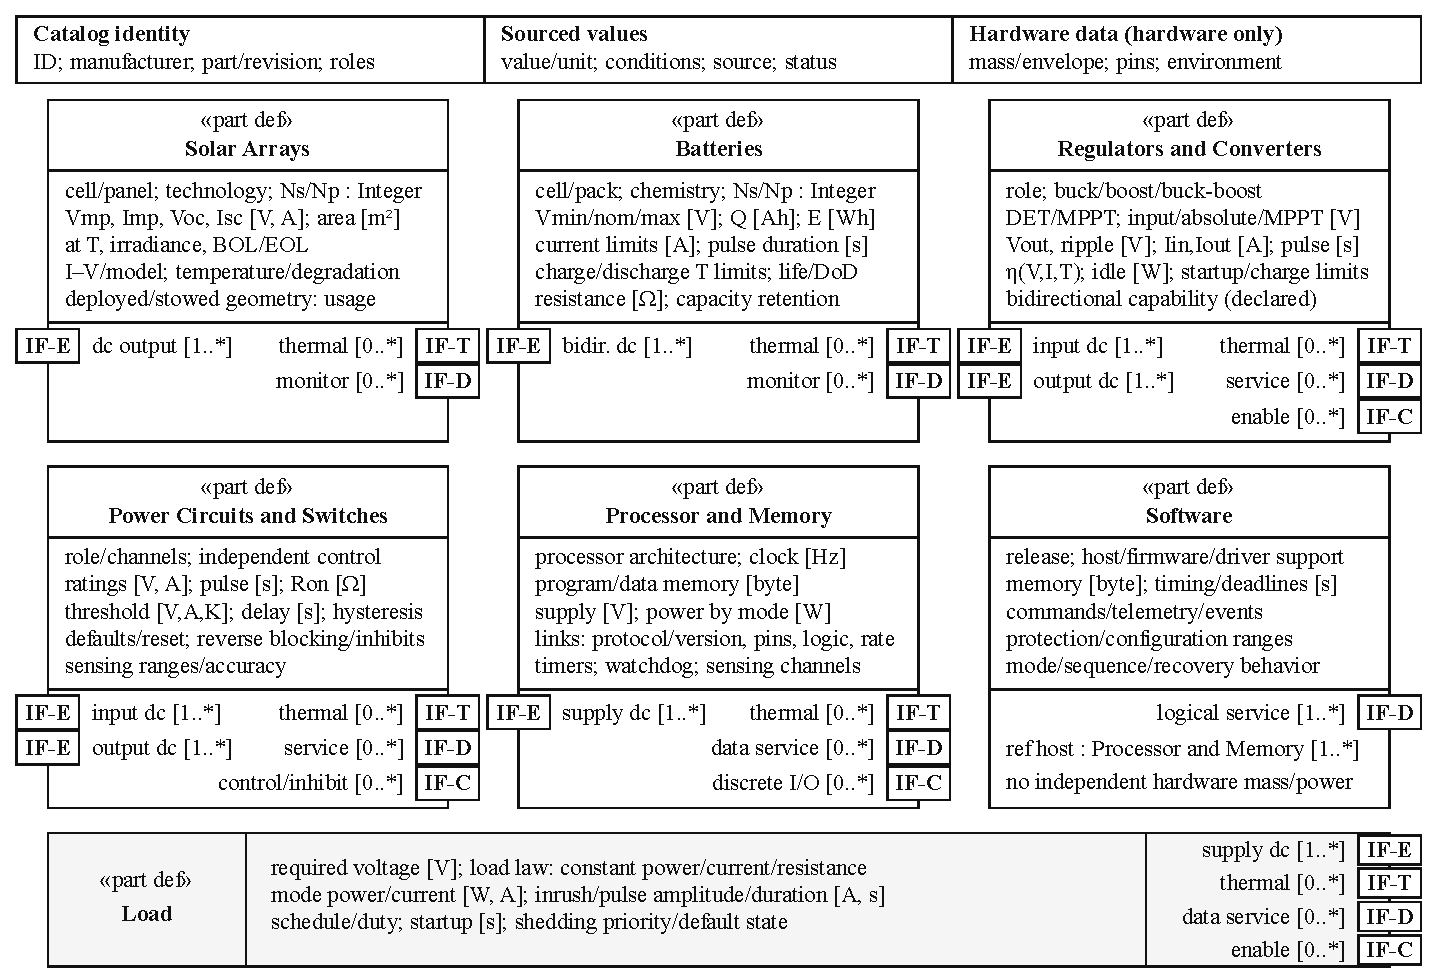
\includegraphics[width=\linewidth,height=\dimexpr\textheight-40pt\relax,keepaspectratio]{fig/eps-component-models.pdf}
\caption[Generic EPS component and load definitions.]{Proposed EPS component and load definitions. Tables~\ref{tab:eps-catalog-records}--\ref{tab:eps-specialized-properties} specify the shared records, port types and properties. Gray identifies external loads.}
\label{fig:eps-component-models}
\end{figure}
\clearpage
\end{landscape}

\subsection{Catalog records and configured part usages}
\label{subsection:eps-catalog-records}

A generic attribute definition will group each structured record in Table~\ref{tab:eps-catalog-records}. Text, Boolean values, enumerations, integers and quantity values will retain their types. Numerical specifications can be scalars, intervals, curves or tables. Quantity values will retain their original units and a consistent internal representation using the SysML v2 quantities and units library. Energy in Wh and charge in Ah will be convertible to J and C. Temperature values will retain their scale. Counts will be integers and efficiencies and duty fractions will be dimensionless.

Every specification will distinguish minimum, typical, maximum, measured and estimated values. Its conditions will identify applicable temperature, irradiance, lifetime, radiation exposure, state of charge, load and pulse duration. A model reference will identify its parameters, validity domain and supported effects. The status of a field will be available, missing or not applicable, with rationale for the latter two. Each required property will have one specification record. An absent value will retain its missing or not-applicable status. Curves and tables will identify independent variables, dependent quantities and interpolation domains. Optional model data will support progressively richer assessments. Missing data will remain visible in catalog browsing and in the scope of any resulting assessment.

{\small
\setlength{\tabcolsep}{4pt}
\renewcommand{\arraystretch}{1.08}
\begin{longtable}{@{}>{\raggedright\arraybackslash}p{0.22\linewidth}>{\raggedright\arraybackslash}p{\dimexpr0.78\linewidth-2\tabcolsep\relax}@{}}
\caption{Shared catalog and configuration records.}\label{tab:eps-catalog-records}\\
\toprule
\textbf{Record} & \textbf{Fields and meaning} \\
\midrule
\endfirsthead
\toprule
\textbf{Record} & \textbf{Fields and meaning} \\
\midrule
\endhead
\bottomrule
\endfoot
Catalog entry & Record identifier and revision, manufacturer, part number, variant, product revision, product level (cell, component, assembly, board or software), provided functions and CSRM roles, included components, supported configurations and compatible accessories. Procurement fields contain supplier, dated price, currency, availability, lead time and lifecycle status. Software entries also identify release, license and supported host/driver versions. \\
Sourced specification & Property identifier, typed value or bound/table, unit and original representation, value meaning, reference conditions, source document/revision/location, observation or retrieval date, uncertainty and review disposition. A numerical model additionally identifies its equations or curves, parameter set and validity domain. \\
Hardware properties & Mass (kg), envelope dimensions (m), keep-out and mounting geometry, connector and terminal pin maps, operating/storage temperature limits (K), thermal contacts and applicable thermal model. Qualification and radiation records identify tested article/revision, conditions, exposure, outcomes and evidence. Flight heritage is recorded with its configuration and environment. \\
Accounting boundary & For each mass, volume, price or consumption specification, identify whether it covers the complete product or named internal components. Record included consumers and losses. Assemblies retain their own identity and references to their contents. Software physical resources belong to its host. \\
Configured usage & Unique installed-part identity, catalog-entry revision, quantity, supported configuration and settings, location/orientation, deployment state, selected ports and function/requirement allocations. Array placement includes active face normals, usable area and packing fraction. Load and software assignments identify their supplying channel and execution host, respectively. \\
Connection & Endpoint identities and physical terminal/return mapping, harness or adapter identity, resistance (\(\Omega\)) and current rating (A) under stated conditions. Data connections add protocol/version, endpoint roles, signal levels, rate (bit/s), addressing and timing. Discrete lines add polarity, default/fault state and inhibit logic. Each physical auxiliary item has its own usage or an identified assembly accounting boundary. \\
Mission scenario & Orbit and attitude history, illumination, temperatures or thermal boundary conditions, lifetime case, load modes and schedules, allowed transitions, initial battery state, discharge/reserve criteria, assessment duration and energy-closure tolerance (J). Allocations identify mass, volume, installation envelope, cost and required service behavior. Each scenario and criterion retains its source and revision. Assessment scope identifies lifecycle phase, intended use, required evidence and accepted modeling assumptions. \\
\end{longtable}
}

Catalog definitions will separate supported configurations from installed choices. A finished panel or battery pack will retain its fixed internal arrangement. A configurable product will expose only the arrangements supported by its supplier. An assembly built from catalog cells will identify the cells and additional protection, interconnects and packaging. Its resulting characteristics will be derived at the assembly level. Individual component records will remain browseable alongside complete EPS boards.

\subsection{Reusable interface definitions}
\label{subsection:eps-port-types}

Table~\ref{tab:eps-port-types} specifies four reusable interface types. Separate SysML v2 port and interface definitions will specify each entry's endpoints and connection constraints. Their identifiers are local to the EPS design model and distinct from the framework interfaces in Chapter~\ref{ch:solucion}. Each interface usage will connect declared port usages. Physical endpoint descriptions will retain the connector, pin and return mapping. A software service will bind to its host's physical endpoint. A product can provide no data interface, as with a passive cell. Port multiplicities will be resolved for the selected product and configuration.

{\small
\setlength{\tabcolsep}{4pt}
\renewcommand{\arraystretch}{1.08}
\begin{longtable}{@{}>{\raggedright\arraybackslash}p{0.22\linewidth}>{\raggedright\arraybackslash}p{\dimexpr0.78\linewidth-2\tabcolsep\relax}@{}}
\caption{EPS port and interface types.}\label{tab:eps-port-types}\\
\toprule
\textbf{Type} & \textbf{Port features and interface meaning} \\
\midrule
\endfirsthead
\toprule
\textbf{Type} & \textbf{Port features and interface meaning} \\
\midrule
\endhead
\bottomrule
\endfoot
IF-E: electrical & A DC terminal pair has voltage \(v\) (V) relative to its declared return, current \(i\) (A) positive into its owner, source/sink/bidirectional capability, and operating and absolute limits. An ideal interface relates across voltages and through currents. Harnesses, switches, converters and isolating devices retain their own voltage drops and return relationships. \\
IF-T: thermal & A thermal boundary has temperature \(T\) (K), heat flow \(\dot Q\) (W) positive into its owner, and contact/boundary identity. Thermal contacts and models specify resistance or conductance and applicable boundary conditions. The catalog records supported thermal contacts separately from mission temperatures. \\
IF-D: data service & A provider receives Command and Configuration items and emits Telemetry and Event items. A requester uses the conjugated directions. Item definitions contain identifier, target/channel, payload types, quantities/units, permitted ranges, time/validity meaning and applicable sampling, response or deadline criteria. Hardware transport records contain protocol/version, pin mapping, electrical levels, rate, endpoint roles and address. Software refers to that transport through its host. \\
IF-C: discrete control & A directed control, enable or inhibit signal has logical meaning, electrical input/output limits, polarity, pin/return mapping, default and fault state, response time and applicable inhibit truth table. Hardware protection and flight inhibits retain their authority and autonomy from software commands. \\
\end{longtable}
}

\subsection{Component and load properties}
\label{subsection:eps-specialized-properties}

Table~\ref{tab:eps-specialized-properties} gives the specialized attributes and port usages. Product levels, chemistries, topologies, modes, load laws and reset policies will use enumerations. Counts and memory sizes will use integers. Capabilities will use Boolean values or sets of named options. Versions and document identifiers will use text. Configurations, channels, tasks and geometry will use structured records or collections with declared multiplicities. Every numerical characteristic uses the record for sourced specifications. Temperature and lifetime dependence can be represented by bounded tables or applicable models. A property used for preliminary sizing can therefore be replaced by richer characterized data while preserving its quantity, source and interface meaning.

{\small
\setlength{\tabcolsep}{4pt}
\renewcommand{\arraystretch}{1.08}
\begin{longtable}{@{}>{\raggedright\arraybackslash}p{0.22\linewidth}>{\raggedright\arraybackslash}p{\dimexpr0.78\linewidth-2\tabcolsep\relax}@{}}
\caption{Specialized EPS component and load definitions.}\label{tab:eps-specialized-properties}\\
\toprule
\textbf{Definition} & \textbf{Attributes and port usages} \\
\midrule
\endfirsthead
\toprule
\textbf{Definition} & \textbf{Attributes and port usages} \\
\midrule
\endhead
\bottomrule
\endfoot
Solar Arrays & Product level, cell technology, supported series/parallel counts \(N_s,N_p\), active area \(A\) (m\(^{2}\)), \(V_{\mathrm{mp}},V_{\mathrm{oc}}\) (V), \(I_{\mathrm{mp}},I_{\mathrm{sc}}\) (A), current--voltage/model data and temperature/degradation characteristics at identified beginning/end-of-life conditions. Panel definitions identify independent sections, bypass/reverse-blocking features and supported deployment states. Installed orientation and packing belong to the usage. Ports: DC output IF-E [1..*], thermal IF-T [0..*] and monitoring IF-D [0..*]. \\
Batteries & Product level, chemistry, supported \(N_s,N_p\), minimum/nominal/maximum voltage (V), rated charge \(Q\) (C, commonly Ah), rated energy \(E\) (J, commonly Wh), charge/discharge current limits (A) with pulse durations (s), separate charging/discharging temperature limits, cycle-life versus DoD data, retained-energy/charge factors \(f_E,f_Q\), energy efficiencies \(\eta_c,\eta_d\), coulombic efficiencies \(\eta_{Q,c},\eta_{Q,d}\), internal resistance (\(\Omega\)) and voltage/discharge model. Pack features identify balancing, protection, sensing and heaters included in the product. Ports: bidirectional DC IF-E [1..*], thermal IF-T [0..*] and monitoring IF-D [0..*]. \\
Regulators and Converters & Conversion/charging roles, buck/boost/buck--boost/linear or direct-transfer implementation, DET/MPPT capabilities, input operating interval and absolute limit (V), tracking interval (V), permissible source current (A), output voltage/ripple (V), continuous/pulse input and output limits (A, s), startup conditions and conversion envelope \(\mathcal C\). Loss or efficiency maps \(P_{\mathrm{loss}}\), \(\eta\) identify voltage, current, temperature, mode and whether idle power \(P_0\) (W) is included. Charger data identify chemistry, supported cell counts, voltage/current limits, termination and temperature rules. Ports: DC input and output IF-E [1..*] each, with reverse transfer explicitly declared, thermal IF-T [0..*], service IF-D [0..*] and enable IF-C [0..*]. \\
Power Circuits and Switches & Circuit role, channel count and independently controlled/protected groups, default states, voltage and continuous/pulse current ratings (V, A, s), on resistance (\(\Omega\)), idle power (W), sensing ranges/accuracy, reverse-current blocking and supported inhibits. Protection data contain threshold bounds (V, A, K), trip-time curves (s), hysteresis, safe operating area, reset/retry policy and hardware/software responsibility. The usage sets values within these supported ranges. Ports: DC input and output IF-E [1..*] each, thermal IF-T [0..*], service IF-D [0..*] and control/inhibit IF-C [0..*]. Harness records use the applicable circuit and connection properties. \\
Processor and Memory & Processor architecture, clock rate (Hz), available program/data memory (byte), supply interval (V), consumption by mode (W), physical link definitions, timers, watchdog and sensing/input/output channel capabilities. Resource availability identifies reservations by supplied firmware. Ports: supply IF-E [1..*], thermal IF-T [0..*], service IF-D [0..*] and discrete input/output IF-C [0..*]. \\
Software & Release, compatible host/firmware/driver versions, required program/data memory (byte), task periods, execution bounds and deadlines (s) for the declared host, supported commands/telemetry/events, parameter ranges, mode transitions, sequencing, shedding and recovery behavior. A reference identifies execution hosts of type Processor and Memory [1..*] and task/resource allocations. Logical service ports are IF-D [1..*]. Physical mass, electrical consumption and thermal dissipation are assigned to the host. \\
Load & Required supply interval (V), load law (constant power, constant current, resistance or characterized curve), \(P_{\ell m}\) (W), \(I_{\ell m}\) (A) or \(R_{\ell m}\) (\(\Omega\)) by mode \(m\), startup/pulse amplitude and duration (A, s), startup time (s), schedule/duty fraction, default state, shedding priority and essential-service constraints. Heat dissipation or a thermal model identifies the thermal load. Startup/pulse intervals identify whether they replace or supplement steady consumption. Ports: supply IF-E [1..*], thermal IF-T [0..*], service IF-D [0..*] and enable IF-C [0..*]. \\
\end{longtable}
}

\section{EPS Component Selection}
\label{section:eps-component-selection}

Selection will operate on the definitions in Section~\ref{section:eps-generic-models}. Jacobs and Selva provide forward evaluation of selected products and backward enumeration of catalog combinations, with critical requirements filtering the feasible set before cost comparison \citep[Sec.~2]{citation-1136}. Wijaya et al. contribute architecture choices and dependencies followed by numerical evaluation \citep[Secs.~4.1--4.4]{review-0055}. Their COTS study distinguishes fixed purchased properties from continuously sized components \citep[Sec.~III]{review-0145}. GREATCUBE+ contributes repeated compatibility assessment after component replacement \citep[Secs.~2.2.1--2.2.2]{review-0711}. Boan contributes the electrical configuration and mission energy-balance iteration \citep[Secs.~3--4]{review-0289}. The following equations and algorithm synthesize these contributions for the proposed schema. Applicable criteria and evidence levels will follow the declared lifecycle phase and intended use. Preliminary electrical feasibility and component qualification will retain distinct assessment scopes.

\subsection{Catalog browsing and architecture alternatives}

Browsing will support filters for CSRM role, product level, manufacturer, supported topology, electrical ranges, environmental conditions, physical envelope, interfaces and procurement constraints. Results will expose the source and conditions of each compared value. Unknown properties will be shown separately from known violations. A typical rating will establish no guaranteed limit unless an engineer accepts a sourced conservative bound. Datasheet maxima, operating limits and measured performance will retain their distinct meanings.

A candidate \(d\) will comprise topology choices, catalog revisions, integer quantities, supported configurations, connections, assignments of loads to channels and allocations of software to hosts. Topology choices will follow Figure~\ref{fig:csrm-eps-topology}: DET or MPPT conditioning, centralized or distributed transfer, bus regulation, and direct or converted supply for each output rail. Direct and converted outputs can coexist. Product capabilities and dependencies will restrict these combinations. Required functions, external controller circuitry and auxiliaries must be covered by identified installed usages. Logical role coverage alone will establish no current capacity, fault independence or geometric fit.

Finished product properties will remain fixed during selection. Series/parallel changes will be permitted for configurable products and assemblies of catalog cells. Supplier configurations or engineer-declared assembly bounds will keep the enumeration finite. A product substitution will trigger renewed sizing, loss, interface and scenario assessments. New conditions or load schedules will remain explicit scenario revisions.

\subsection{Generation and storage configuration}

Equations~\eqref{eq:minimum-panel-power}--\eqref{eq:battery-energy} will provide preliminary screens for each candidate. The solar cell count will be recalculated from the selected cell's EOL data and rounded upward for physical assembly. For identical cells distributed over sections \(g\), the installed count will satisfy the preliminary lower bound
\begin{equation}
    \sum_g N_{s,g}^{\mathrm{pv}}N_{p,g}^{\mathrm{pv}}\geq\left\lceil N_{\mathrm{sc}}\right\rceil,
    \qquad N_{s,g}^{\mathrm{pv}},N_{p,g}^{\mathrm{pv}}\in\mathbb Z_{>0}.
    \label{eq:pv-integer-configuration}
\end{equation}
Sections on differently illuminated faces will be evaluated separately. Installed cell count will be followed by an illumination-dependent generation assessment. With irradiance, temperature and orientation from scenario \(\sigma\), the selected current--voltage model and operating point give each section's available source power \(P_{g,\mathrm{avail}}(t,\sigma)\). At the same source boundary as Equation~\eqref{eq:minimum-panel-power}, a screen using average power during sunlight is
\begin{equation}
    \frac{1}{T_s}\int_{\mathrm{sunlight}}\sum_g P_{g,\mathrm{avail}}(t,\sigma)\,dt
    \geq P_{\mathrm{sp}_{\min}}.
    \label{eq:array-generation-screen}
\end{equation}
This screen will use the candidate's attainable operating point under DET or MPPT and its applicable path efficiencies \(X_s,X_e\). Stored energy, charge acceptance and load peaks will be assessed separately below.

For a matched section connected to MPPT input \(r\), the following conservative checks will use extrema over the applicable temperature, irradiance and lifetime conditions:
\begin{align}
    [N_s^{\mathrm{pv}}V_{\mathrm{mp}}^{\mathrm{lo}},
     N_s^{\mathrm{pv}}V_{\mathrm{mp}}^{\mathrm{hi}}]
    &\subseteq[V_{\mathrm{track},r}^{\mathrm{lo}},V_{\mathrm{track},r}^{\mathrm{hi}}],
    \label{eq:mppt-voltage-compatibility}\\
    N_s^{\mathrm{pv}}V_{\mathrm{oc}}^{\mathrm{hi}}&\leq V_{\mathrm{abs},r},
    \qquad N_p^{\mathrm{pv}}I_{\mathrm{sc}}^{\mathrm{hi}}\leq I_{\mathrm{source,allow},r}.
    \label{eq:pv-input-ratings}
\end{align}
Here \(V_{\mathrm{abs},r}\) is the absolute input limit and \(I_{\mathrm{source,allow},r}\) is the permissible source current from the converter specification. Startup and operating-voltage limits will also be checked. Shared trackers will require a compatible combined current--voltage characteristic. DET configurations will instead use the array characteristic at the battery/bus operating voltage, including blocking and wiring drops.

For an assembly of identical battery cells, the initial estimates will be
\begin{equation}
    \begin{aligned}
        E_{\mathrm{pack,BOL}}&=N_s^{\mathrm{bat}}N_p^{\mathrm{bat}}E_{\mathrm{cell,BOL}},\\
        Q_{\mathrm{pack,BOL}}&=N_p^{\mathrm{bat}}Q_{\mathrm{cell,BOL}}.
    \end{aligned}
    \label{eq:battery-assembly-capacity}
\end{equation}
\begin{equation}
    \begin{aligned}
        \relax[V_{\mathrm{pack}}^{\mathrm{lo}},V_{\mathrm{pack}}^{\mathrm{hi}}]
        &=[N_s^{\mathrm{bat}}V_{\mathrm{cell}}^{\mathrm{lo}},N_s^{\mathrm{bat}}V_{\mathrm{cell}}^{\mathrm{hi}}],\\
        I_{\mathrm{pack,allow}}&=N_p^{\mathrm{bat}}I_{\mathrm{cell,allow}}.
    \end{aligned}
    \label{eq:battery-assembly-ratings}
\end{equation}
Current limits will retain separate charging, discharging and pulse conditions. The DoD limit will use the selected cell's cycle-life data under applicable conditions. Coefficients \(a,b\) in Equation~\eqref{eq:battery-cycle-life} will retain their sourced fit domain. Packaging, interconnects, balancing and protection can further restrict these cell-based estimates. A finished pack will use its supplier's pack ratings. The preliminary capacity screen will compare \(E_{\mathrm{pack,BOL}}\) with \(E_{\mathrm{Battery}}\). EOL assessment will use the specified retained capacity or an applicable aging model, with \(E_{\mathrm{pack,EOL}}=f_EE_{\mathrm{pack,BOL}}\) where that factor is valid. Margin \(M\) will be applied once in preliminary sizing. The physical EOL model will use retained capacity without applying \(M\) again. The selected chemistry, cell count, charging voltage/current, temperature restrictions and termination rules will be matched to the charger.

\subsection{Connections, loads and operating limits}

At an ideal IF-E connection, consistent terminal and return mapping will give
\begin{equation}
    v_a=v_b,\qquad i_a+i_b=0.
    \label{eq:electrical-interface-conservation}
\end{equation}
Current is positive into each connected part. A physical path will include its declared losses. For a resistive supply-and-return path,
\begin{equation}
    V_\ell=V_r-I_{\mathrm{path}}R_{\mathrm{path}},
    \label{eq:load-path-drop}
\end{equation}
where \(V_r\) is the supplying rail voltage and \(R_{\mathrm{path}}\) includes the relevant harness, contact and conducting-switch resistance once. Shared paths will carry the sum of their branch currents. Isolation and differing returns will require an explicitly modeled interface or adapter.

The load law in Table~\ref{tab:eps-specialized-properties} will determine current at the actual terminal voltage:
\begin{equation}
    I_\ell(V_\ell,m)=
    \begin{cases}
        P_{\ell m}/V_\ell, & \text{constant power},\\
        I_{\ell m}, & \text{constant current},\\
        V_\ell/R_{\ell m}, & \text{resistive load}.
    \end{cases}
    \label{eq:generic-load-law}
\end{equation}
A characterized load will use its supplied curve or model instead. Mode schedules and pulse records will identify simultaneous demand. For every active load and applicable scenario,
\begin{equation}
    V_\ell^{\mathrm{req,lo}}\leq V_\ell(t,\sigma)\leq V_\ell^{\mathrm{req,hi}},
    \qquad
    \sum_{\ell\in\mathcal L_r}I_\ell(t,\sigma)
    \leq I_{r,\mathrm{allow}}(T,\text{duration}).
    \label{eq:rail-load-compatibility}
\end{equation}
\(\mathcal L_r\) contains loads assigned to rail or channel \(r\). Shared channel groups and converter inputs will be checked against their aggregate ratings. Continuous operation and startup/pulse events will use their respective limits. A converter's operating tuple \((V_{\mathrm{in}},V_{\mathrm{out}},I_{\mathrm{out}},T)\) must lie within its sourced conversion envelope \(\mathcal C_r\). This will include dropout, conversion-ratio and startup restrictions.

Demand will be propagated upstream through the selected paths using
\begin{equation}
    P_{\mathrm{in},r}=P_{\mathrm{out},r}+P_{\mathrm{loss},r}.
    \label{eq:conversion-loss-accounting}
\end{equation}
An efficiency specification implies \(P_{\mathrm{loss},r}=P_{\mathrm{out},r}(\eta_r^{-1}-1)\) within its stated domain. Separate idle power will be added only when excluded from that efficiency. Zero-load and disabled states will use their own consumption data. An aggregate board-input specification and its included internal loads will contribute once. The same rule will prevent software execution from becoming an additional physical load alongside its host.

Protection assessment will compare legitimate steady and pulse demand with the no-trip region, then compare fault interruption with the protected path's current, energy and safe-operating-area limits. Threshold tolerances and interruption times will be evaluated together against the protected path's continuous, pulse and safe-operating-area limits. Pulse tolerance, trip delay, hysteresis, retry and default states will be checked separately. Declared hardware protection and flight inhibits must remain effective under the specified processor/software failure conditions.

Hardware temperatures will remain within the applicable operating intervals. Battery charging and discharging will use their distinct temperature restrictions. Qualification and radiation evidence will be assessed against the mission environment and exact product configuration. An environmental evidence gap will remain an unresolved assessment, with no inferred qualification from flight heritage alone.

IF-D and IF-C checks will compare directed features, quantities, identifiers, pin assignments, logic levels, protocols, versions, address allocation, timing and startup/fault behavior. A common connector shape or protocol name will establish no complete compatibility. Software-host checks will include architecture, supplied firmware and drivers, available memory and execution assumptions. For tasks \(a\) allocated to host \(h\), preliminary resource screens will be
\begin{equation}
    \sum_{a\in\mathcal A_h}B_a^{\mathrm{data}}\leq B_h^{\mathrm{available}},
    \qquad
    \sum_{a\in\mathcal A_h}\frac{C_a}{T_a}\leq U_h^{\mathrm{allocated}},
    \label{eq:software-resource-screen}
\end{equation}
where \(B_a^{\mathrm{data}}\) is required data memory, \(C_a\) is execution time on the declared host, \(T_a\) is task period and \(U_h^{\mathrm{allocated}}\) is the allocated processor utilization. Program storage will be checked similarly. These screens will establish no deadline guarantee. Scheduling and service-response evidence will be assessed against the declared deadlines. Supplied opaque firmware will require applicable vendor or assessment evidence for the claimed services and timing.

\subsection{Mission energy balance and resource budgets}

Surviving configurations will be assessed over the mission scenarios using their selected component models. Solar geometry, temperature, battery voltage, converter operating points and loss maps will remain coupled. At a common reference boundary outside the battery terminals, let \(P_g\) be solar power available after conditioning and \(P_d\) the upstream demand of all loads and distribution paths, including EPS consumption. Both powers will include the applicable external path losses. Battery internal losses will be represented by its efficiencies or selected battery model. The net available power is \(P_\Delta=P_g-P_d\). A preliminary energy model will use
\begin{align}
    P_{\mathrm{dis},k}&=\max(-P_{\Delta,k},0),
    \label{eq:battery-discharge-demand}\\
    P_{\mathrm{ch},k}&=\min\left\{\max(P_{\Delta,k},0),\,
    P_{\mathrm{ch,allow},k},\,
    \frac{E_{\max}-E_k}{\eta_{c,k}\Delta t},\,
    \frac{v_{b,k}(Q_{\max}-Q_k)}{\eta_{Q,c}\Delta t}\right\},
    \label{eq:battery-charge-acceptance}\\
    E_{k+1}&=E_k+\left(\eta_{c,k}P_{\mathrm{ch},k}
    -\frac{P_{\mathrm{dis},k}}{\eta_{d,k}}\right)\Delta t.
    \label{eq:battery-energy-propagation}
\end{align}
Here energy is in J, power in W and \(\Delta t\) in s. \(v_{b,k}\) is battery terminal voltage at step \(k\). \(E_{\max}\) is a conservative fixed energy capacity for the run's temperature/lifetime case. Charge acceptance \(P_{\mathrm{ch,allow}}\) will include battery and charger voltage, current, temperature and termination limits. Unused solar surplus will follow the selected circuit's curtailment or shunt capability. Resulting voltage and heat will be assessed. Required discharge above a battery or path limit will be a failure. Energy shortages will be retained as failures. Assessment will stop at an invalid battery state. Terminal-voltage and transient assessments will use the applicable battery and circuit models.

Charge-based state of charge \(z\) will remain distinct from normalized stored energy. With battery-port current \(i_b\) positive into the battery, a coulomb-counting model will use
\begin{equation}
    \begin{aligned}
        Q_{k+1}&=Q_k+\left(\eta_{Q,c}\max(i_{b,k},0)
        -\frac{\max(-i_{b,k},0)}{\eta_{Q,d}}\right)\Delta t,\\
        z_k&=Q_k/Q_{\max}.
    \end{aligned}
    \label{eq:battery-charge-propagation}
\end{equation}
\(Q\) is remaining charge in C and \(Q_{\max}\) is its applicable retained capacity. Current will be obtained from the battery terminal voltage and charge/discharge power. The energy and charge models will require consistent characterized data, including their respective efficiencies. Full-charge limits will constrain both states. A richer battery model can replace these preliminary balances while retaining the same interface and loss boundaries. An energy-only assessment will leave charge-based DoD and voltage criteria unassessed without an applicable mapping.

For nominal repeating conditions, the criteria will include
\begin{equation}
    z_k\geq1-\mathrm{DoD}_{\max},\qquad
    E_{\mathrm{end}}\geq E_{\mathrm{start}}-\epsilon_E,
    \label{eq:nominal-energy-feasibility}
\end{equation}
with declared initial state and numerical energy-closure tolerance \(\epsilon_E\). Survival and recovery cases will use their own allowed duration, initial state, essential loads and minimum reserve. They will retain any authorized exceptional discharge separately from nominal cycle-life criteria. Load shedding will follow the declared service and priority constraints.

For uniquely accounted physical or procurement usages \(j\), quantity \(q_j\) will give
\begin{equation}
    \begin{aligned}
        m_{\mathrm{EPS}}&=\sum_jq_jm_j\leq m_{\mathrm{allocated}},\\
        V_{\mathrm{occupied}}&=\sum_jq_jV_j\leq V_{\mathrm{allocated}},\\
        C_{\mathrm{EPS}}&=\sum_jq_jc_j+C_{\mathrm{additional}}.
    \end{aligned}
    \label{eq:eps-product-budgets}
\end{equation}
\(m_j,V_j,c_j\) denote product mass, occupied envelope volume and unit price, respectively. The budget will include required harnesses, adapters, packaging and protection. \(C_{\mathrm{additional}}\) will contain separately declared integration, licensing or qualification costs excluded from product prices. Currency conversion will retain its rate and date. Missing prices or effort estimates will limit the cost comparison. Volume totals will be followed by installation-envelope, keep-out, mounting, connector-access and stack-height checks. Aggregate and internal component properties will follow their accounting boundaries independently for each budget.

\subsection{Parametric EPS requirements}
\label{subsection:eps-parametric-requirements}

Table~\ref{tab:eps-parameter-requirements} proposes requirements on the modeled EPS and its service to the loads. They synthesize the cited design methods using the properties in Tables~\ref{tab:eps-catalog-records}--\ref{tab:eps-specialized-properties}. Component and load limits, allocations and supplied scenarios determine the criteria. The requirements apply to the selected functions and configurations across their specified modes, temperatures, illumination, lifetime cases, schedules and pulses. Bounded calculations and supplied histories can support concept assessment through MR-03. Steady, pulse and state bounds suffice where they establish the predicates. More detailed model and software assessments can refine these results in MR-04--06.

A requirement passes when its predicate holds throughout the applicable conditions. A known violation fails. Missing decisive parameters or bounds spanning compliance and violation leave the assessment unassessed. An absent optional function is not applicable. Operating limits and absolute maxima retain their separate meanings. Pulse records determine whether startup demand replaces or supplements steady consumption. The symbol \(z_{\min,\sigma}\) denotes the minimum charge-based state of charge permitted by scenario \(\sigma\), including its applicable discharge and reserve criteria. Energy reserve criteria apply directly to stored energy.

\begingroup
\small
\setlength{\tabcolsep}{4pt}
\setlength{\parskip}{0pt}
\setlength{\LTpre}{0.4\baselineskip}
\setlength{\LTpost}{0.4\baselineskip}
\renewcommand{\arraystretch}{1.06}
\setlength{\ReportTableBodyWidth}{\dimexpr\linewidth-6\tabcolsep\relax}
\begin{longtable}{@{}P{0.09\ReportTableBodyWidth}P{0.37\ReportTableBodyWidth}P{0.29\ReportTableBodyWidth}P{0.25\ReportTableBodyWidth}@{}}
\caption{Parameter-based EPS and load requirements.}\label{tab:eps-parameter-requirements}\\
\toprule
\textbf{ID} & \textbf{Requirement and equation or algorithm} & \textbf{Pass/fail criterion} & \textbf{Rationale} \\
\midrule
\endfirsthead
\toprule
\textbf{ID} & \textbf{Requirement and equation or algorithm} & \textbf{Pass/fail criterion} & \textbf{Rationale} \\
\midrule
\endhead
\bottomrule
\endfoot
\multicolumn{4}{@{}l}{\textbf{Configuration and power paths}} \\*
EPS-01\phantomsection\label{epsreq:EPS-01} & The EPS shall use supported product configurations and settings. Compare each configured usage, including series/parallel counts, with its supported options or declared cell-assembly bounds and required external circuitry. & Every choice is supported. Configured cell counts are positive integers. Required external circuits and adapters are included. Finished panels and packs retain their fixed properties and internal arrangement. & Purchased products constrain realizable configurations \citep[Sec.~III.A--B]{review-0145}. \\
EPS-02\phantomsection\label{epsreq:EPS-02} & The solar arrays shall meet the preliminary generation bound in Equation~\eqref{eq:array-generation-screen}. Assemblies of identical cells shall also meet Equation~\eqref{eq:pv-integer-configuration}. & The sunlight generation bound holds at the attainable DET or MPPT operating point under the applicable illumination and EOL conditions. Applicable cell-count bounds hold. This screen is additional to EPS-10--12. & Illumination, operating point and EOL properties determine usable generation \citep[Secs.~3--4]{review-0289}. \\
EPS-03\phantomsection\label{epsreq:EPS-03} & The solar-array connections shall remain within the receiving input limits. Apply Equations~\eqref{eq:mppt-voltage-compatibility} and~\eqref{eq:pv-input-ratings} where applicable. For DET or shared trackers, compare the combined current--voltage characteristic at the selected operating point with the supported input range. & Operating and startup voltages remain supported. Open-circuit voltage and permissible source current satisfy their separate limits. MPPT tracking bounds and shared-input characteristics are compatible where selected. & Temperature and panel arrangements affect electrical compatibility \citep[Secs.~3--4]{review-0289}\citep[Sec.~7.1]{handpicked-0003}. \\
EPS-04\phantomsection\label{epsreq:EPS-04} & Each converter shall supply its assigned rail within its conversion envelope \(\mathcal C_r\). Compare its operating tuples with that envelope, including startup, dropout and conversion-ratio restrictions. & Every required operating tuple is supported. The converter starts at the required source condition and supplies the required output voltage and current. & Converter topology restricts attainable supply conditions \citep[Sec.~4]{handpicked-0003}. \\
EPS-05\phantomsection\label{epsreq:EPS-05} & Each charger shall support the selected battery chemistry, series count and charge policy. Compare these settings with battery and charger limits, then apply Equation~\eqref{eq:battery-charge-acceptance}. & Chemistry and cell count are supported. Charging voltage, current and termination satisfy both battery and charger rules, including charging-temperature restrictions in EPS-13. & Battery charging and regulator modes must be compatible \citep[Secs.~2.2--2.3]{review-0573}. \\
EPS-06\phantomsection\label{epsreq:EPS-06} & The EPS shall maintain each load's terminal voltage within its supply interval whenever its service is required. Apply Equations~\eqref{eq:load-path-drop}--\eqref{eq:rail-load-compatibility}, including battery-voltage bounds and pulses. Evaluate startup against its specified time and supply conditions. & Voltage limits hold throughout required service and applicable pulse intervals. Startup reaches the specified service state within the allowed time. Returns, isolation and adapters provide the required voltage relationship. & Battery and distribution drops affect load supply voltage \citep[Secs.~2.3--2.4]{review-0573}. \\
EPS-07\phantomsection\label{epsreq:EPS-07} & The EPS shall supply simultaneous steady and pulse demand within battery, converter, switch and connection current limits. Propagate power upstream with Equation~\eqref{eq:conversion-loss-accounting}, derive current at each path's voltage and sum shared-path currents. & Every input, output and shared path satisfies its continuous or pulse rating at the applicable temperature and duration. Battery charge and discharge limits remain distinct. Included consumers, losses and host execution consumption contribute once. & Coincident loads can exceed EPS current limits despite adequate average energy \citep[Sec.~VI]{review-1231}. \\
\multicolumn{4}{@{}l}{\textbf{Storage and mission energy}} \\*
EPS-08\phantomsection\label{epsreq:EPS-08} & The battery pack shall meet the preliminary capacity in Equation~\eqref{eq:battery-energy}. Derive cell-assembly ratings with Equations~\eqref{eq:battery-assembly-capacity}--\eqref{eq:battery-assembly-ratings}, or use finished-pack ratings. Use retained energy and charge in the lifetime cases. & \(E_{\mathrm{pack,BOL}}\geq E_{\mathrm{Battery}}\). Applicable EOL capacities are \(E_{\max}=f_EE_{\mathrm{pack,BOL}}\) and \(Q_{\max}=f_QQ_{\mathrm{pack,BOL}}\). Margin \(M\) enters preliminary sizing once and is not reapplied to retained capacity. Scenario sufficiency also requires EPS-10--12. & Eclipse demand and degradation constrain battery capacity \citep[Secs.~3 and~6.2.2]{handpicked-0003}. \\
EPS-09\phantomsection\label{epsreq:EPS-09} & The battery pack shall support the required nominal cycling within the selected cycle-life limits. Compare Equation~\eqref{eq:battery-mission-cycles} with the cell or pack cycle-life data at the selected DoD and operating conditions. Use Equation~\eqref{eq:battery-cycle-life} only within its applicable fit domain. & Supported cycle life is at least \(N_{\mathrm{cycle}}\). Nominal cycle DoD does not exceed \(\mathrm{DoD}_{\max}\). Exceptional survival discharge uses its separate scenario limit. & Cycle life depends on discharge depth and operating conditions \citep[Sec.~3]{handpicked-0003}. \\
EPS-10\phantomsection\label{epsreq:EPS-10} & The EPS shall supply the scheduled nominal loads while retaining their required battery reserve. Propagate discharge, accepted charging, energy and charge with Equations~\eqref{eq:battery-discharge-demand}--\eqref{eq:battery-charge-propagation}. Apply the nominal DoD condition in Equation~\eqref{eq:nominal-energy-feasibility} and scenario reserve limits. & All required demand is supplied. At every step, \(0\leq E_k\leq E_{\max}\) and \(0\leq z_{\min,\sigma}\leq z_k\leq1\). Nominal DoD and any energy reserve limits hold. Shortages fail even when orbital average generation exceeds consumption. & Energy histories expose shortages hidden by average budgets \citep[Secs.~V--VI]{review-1231}. \\
EPS-11\phantomsection\label{epsreq:EPS-11} & The EPS shall replenish the battery over each specified nominal repeating interval. Compare the propagated ending energy and charge-based state of charge with their initial values using Equation~\eqref{eq:nominal-energy-feasibility}. & \(E_{\mathrm{end}}\geq E_{\mathrm{start}}-\epsilon_E\) and \(z_{\mathrm{end}}\geq z_{\mathrm{start}}\). Here start and end identify the repeating interval boundaries. The supplied \(\epsilon_E\) is a numerical closure tolerance, not an allowance for persistent energy depletion. & Sustained operation requires generation to replenish consumed storage \citep[Sec.~3]{review-0289}. \\
EPS-12\phantomsection\label{epsreq:EPS-12} & The EPS shall supply essential loads throughout the specified survival interval and support the required recovery. Propagate the scenario's initial state, reduced illumination, load shedding and allowed transitions with the same energy and charge balances. & Essential-load service holds for the required duration. Energy and charge remain within the scenario's reserve and exceptional discharge limits. The specified recovery transition is reached within its allowed duration while satisfying EPS-04--07. & Survival following eclipse can determine battery capacity \citep[Sec.~3, Fig.~11]{review-0289}. \\
EPS-13\phantomsection\label{epsreq:EPS-13} & EPS components shall remain within their operating-temperature intervals. Compare supplied temperature histories or thermal-model bounds with each component's state-dependent limits at the corresponding cell, case or junction reference. Include required heaters as loads in EPS-07 and EPS-10--12. & Component temperature limits hold. Charging occurs only within the charging-temperature interval and discharge respects its separate interval. Required heater demand is supplied with the associated battery and load service. & Temperature restrictions and heater demand affect usable energy \citep[Sec.~6.2.3, Table~4]{handpicked-0003}. \\
EPS-14\phantomsection\label{epsreq:EPS-14} & The EPS shall dispose of available solar surplus through its supported curtailment or shunt behavior. With \(P_{\mathrm{sur},k}\) denoting unused conditioned source power (W), evaluate \(P_{\mathrm{sur},k}=\max(P_{\Delta,k},0)-P_{\mathrm{ch},k}\), including full-charge conditions. & The selected behavior accommodates the surplus within circuit voltage, current and thermal limits while maintaining required load service. Charge termination is respected. Shunted power enters dissipation. Curtailed generation is foregone harvest. & Full charge changes regulator operation and available charging power \citep[Secs.~2.2 and~3.1]{review-0573}. \\
\multicolumn{4}{@{}l}{\textbf{Protection and control states}} \\*
EPS-15\phantomsection\label{epsreq:EPS-15} & The EPS shall interrupt the declared fault currents before protected-path limits are exceeded and supply legitimate demand without nuisance trips. Compare load profiles with the no-trip region and fault current/energy/duration bounds with protected-path ratings and safe operating area. & Legitimate steady and pulse profiles remain in the no-trip region. Threshold tolerances and interruption times together keep fault stress within continuous/pulse ratings and safe operating area. Settings remain within supported protection ranges. & Protection separates legitimate demand from damaging fault stress \citep[Secs.~7.4--7.5 and~8.1.6]{handpicked-0003}. \\
EPS-16\phantomsection\label{epsreq:EPS-16} & The EPS shall enter the specified protective state at battery undervoltage or overvoltage and recover according to its hysteresis and reset policy. Apply the supplied voltage bounds and threshold crossings to the switch states, essential loads and recharge path. & Cutoff and re-enabling follow the threshold bounds, hysteresis and trip/reset delays. Output states, safe-state loads and permitted recharge paths follow the configured policy. Energized loads remain within their applicable supply limits. & Cutoff hysteresis protects the battery and permits recovery \citep[Secs.~7.4 and~8.1.6]{handpicked-0003}. \\
EPS-17\phantomsection\label{epsreq:EPS-17} & The EPS shall realize its specified power-on and inhibited states. Evaluate the applicable IF-C truth table and allowed state transitions with source-voltage bounds, startup conditions and output defaults, including specified processor/software failure states. & Each truth-table combination and allowed transition gives the required output state. Inhibited outputs remain unpowered except for explicitly permitted domains. Required autonomous protection and inhibits remain effective when the processor is unavailable. & Power-on circuitry and adopted deployment constraints define permitted energized states \citep[Sec.~7.6]{handpicked-0003}\citep[Sec.~2.3]{calpoly2022cds}. \\
EPS-18\phantomsection\label{epsreq:EPS-18} & EPS service and control ports shall support the required load-control and monitoring exchanges. Compare connected IF-D and IF-C endpoints for pin/return mapping, direction, identifiers, quantities, signal levels, protocol/version, addresses and required rate or response bounds. & Endpoint meanings and electrical levels are compatible. Addresses are unique where required by the selected transport. Required exchanges fit the supported rates and response bounds. Enable/inhibit polarity and default/fault states match the connected loads. & Telemetry and output control depend on compatible interfaces \citep[Secs.~7.2--7.5]{handpicked-0003}. \\
\multicolumn{4}{@{}l}{\textbf{Physical resource bounds}} \\*
EPS-19\phantomsection\label{epsreq:EPS-19} & The EPS shall remain within its mass and occupied-volume allocations. Apply the mass and volume inequalities in Equation~\eqref{eq:eps-product-budgets} to uniquely accounted usages, including required harnesses, adapters, packaging and protection. & Total EPS mass and occupied volume do not exceed their allocations. Aggregate and internal component values are counted once within their respective accounting boundaries. Geometric accommodation additionally requires EPS-20. & Component budgets must respect allocated resources \citep[Secs.~4--5]{review-0270}. \\
EPS-20\phantomsection\label{epsreq:EPS-20} & The EPS shall fit its allocated installation and array envelopes. Transform configured component envelopes and keep-outs into the installation frame. Compare containment, overlap, mounting, connector access and stack height for each required deployment state. Check cell-assembly area/packing and fixed-panel installation envelopes separately. & Occupied envelopes fit without unintended overlap and keep-outs remain clear. Required mounting and connector access are available. Stack height fits its allocation. For cell assemblies, active cell area does not exceed usable face area multiplied by its packing fraction. & Placement adds geometric constraints beyond volume totals \citep[Sec.~2.3]{review-0711}. \\
\end{longtable}
\endgroup


\subsection{Candidate evaluation and selection algorithm}

Table~\ref{tab:eps-parameter-requirements} supplies the parametric EPS constraints used in this evaluation. Each applicable criterion will return pass, fail or unassessed, with its source, conditions and evidence. Let \(\Sigma\) be the declared scenario set and \(g_i\) its numerical constraint residuals. The feasible set will be
\begin{equation}
    \mathcal F=\left\{d:\ \begin{aligned}
        &g_i(d,\sigma)\leq0\quad\text{for all applicable }i\text{ and }\sigma\in\Sigma,\\
        &\text{all required discrete checks pass,}\\
        &\text{all required assessments are complete and applicable}
    \end{aligned}\right\}.
    \label{eq:eps-feasible-catalog-set}
\end{equation}
Failed convergence or invalid model use will leave the affected criterion unassessed. A known violation will reject the candidate for the declared requirements. Incomplete candidates will remain available for browsing with their missing evidence identified.

Algorithm~\ref{alg:eps-cots-selection} will support both evaluation of an engineer's configuration and generation of catalog alternatives. Enumeration will cover the declared finite discrete choices. Any continuous settings will use a declared evaluation or optimization method inside the supported operating envelope. The method will report the explored scope, convergence and remaining limits. It will make no global-optimum claim for an incomplete search.

\begin{algorithm}[H]
\caption{Proposed EPS catalog evaluation and selection.}
\label{alg:eps-cots-selection}
\begin{algorithmic}[1]
\Require Revisioned catalog, load/scenario records, requirements, allocations and approved comparison criteria.
\State Normalize quantities and retain sources, conditions, accounting boundaries and missing-data states.
\State Retrieve products by required roles and supported capabilities. Retain incomplete matches separately.
\State Generate permitted topology alternatives and bounded product configurations, or accept an engineer's candidate.
\For{each candidate configuration}
    \State Allocate functions, loads, channels, hosts and auxiliaries. Resolve declared ports and connections.
    \State Check supported configurations, function coverage, physical/electrical interfaces and environmental evidence.
    \State Recalculate integer cell arrangements, candidate path losses, sizing and product budgets.
    \State Assess operating limits, protection, software resources, geometry and nominal/survival scenarios.
    \State Record each criterion as pass, fail or unassessed with its evidence and model-validity scope.
    \State Retain feasible candidates, incomplete candidates and rejected candidates with distinct outcomes.
\EndFor
\State Compare feasible candidates on the approved measures and expose their margins and sensitivity.
\State Record the authorized engineer's selection, rationale, exact product/configuration revisions and remaining risks.
\end{algorithmic}
\end{algorithm}

A cost-led comparison will select a minimum-cost member of \(\mathcal F\). A trade study can instead retain non-dominated alternatives for cost, mass and minimum energy reserve above the scenario's required reserve. Preference weights and criteria will be engineer approved. Mandatory failures will exclude a candidate before preference ranking. The selected model will contain a bill of materials, quantities and settings, electrical connections, load/channel and software/host allocations, and links to the requirements and assessments it supports. A catalog match or a passed preliminary screen will retain its analysis scope. It will establish no hardware qualification or completed flight verification.

\subsection{KiCad design handoff}
\label{subsection:eps-kicad-handoff}

The framework will translate current COTS allocations into a KiCad review schematic. It will retain catalog revisions, quantities, sources and one physical usage for each integrated board. Automatic placement and wire routing will connect named logical ports. The drawing will expose missing terminal mappings and will establish no manufacturer circuit reconstruction.

Physical carrier board routing will require reviewed pin and return maps, footprints, approved connectivity, installation geometry and board constraints. The pipeline will freeze the architecture, import approved physical rules, generate board data, exchange routing data with an external autorouter, and retain electrical and design rule reports with unresolved connections.

EPS requirements will inform trace widths, via geometry and spacing through reviewed derivations with declared stackup, thermal conditions, fabrication limits and insulation criteria. KiCad will check supplied connectivity and geometry. Mission energy, operating limits, protection behavior and complete installation fit will retain separate assessments. A board rule pass will leave known EPS failures unchanged and will establish no flight qualification.

\section{EPS Verification and Validation}

\section{System Integration and Verification}
\label{section:integrate-and-verify-system}

The following procedures specify future work. No empirical framework V\&V has run. OOSEM specifies verification subjects, stimuli, conditions, expected responses, verdicts and the enabling verification environment \citep[Secs.~17.3.8--17.3.9]{friedenthal2014practical}. NASA distinguishes requirement conformity from suitability for stakeholder expectations and ConOps. Both can be assessed through inspection, analysis, demonstration or test, with methods suited to product maturity \citep[Secs.~2.4, 5.3--5.4 and Appendix~I]{nasa2016systems}.

The assessment subjects remain distinct. Framework verification checks the implemented framework's FRs. Framework validation checks engineering suitability in representative use. EPS phase-product V\&V checks the engineered concept, requirements, models or host software. Model credibility assesses supported predictions, with calibration kept separate from independent assessment. Research evaluation measures the enterprise MOEs and bounded transfer. Shared observations can support several assessments only when each subject and comparison basis remain explicit.

Qualification assesses an identified future framework configuration or assistance profile. It uses approved criteria within the model and software scope. Hardware and flight qualification remain outside scope.

\subsection{Framework requirement verification}

The subject is an identified implemented framework candidate and core revision. Record component, authoring, rule, corpus, scoring-model, solver, compiler and library versions. Declare the host, workload, access rights, selected analysis tools, F Prime integration profile, reference data, backup and reconstruction arrangements. Verification personnel need the relevant systems, EPS, analysis and software skills. Independent experts establish reference results and adjudicate disagreements separately from development and blind assessment. Ordinary computing, controlled models/data and reviewers form the enabling environment. No physical EPS equipment or testing facility is required.

The Systems Engineer owns this plan and its criteria. This engineer agrees reference answers, intended-use limits, workloads, thresholds and comparison rules with engineers, independent experts and stakeholders at the framework requirements baseline, before qualification. Missing criteria block performance qualification. The designated authority controls baseline and procedure changes. Numerical targets remain to be resolved (TBR). Their risk basis includes missed syntax defects, unsuitable recommendations, incorrect numerical results and incomplete analysis reconstruction. Resolution covers recommendation applicability, change impacts, numerical errors, reconstruction and view interpretation. Fix workloads, thresholds and comparison rules before execution. Recording a TBR supplies no passing verdict \citep[Secs.~6.1.1.2.4 and~6.7]{nasa2016systems}.

\paragraph{Common procedure for every V case.}
(1) Identify the subject, applicable FR, configuration and controlled references. (2) Confirm prerequisites, profile coverage and approved criteria. Record missing inputs or unresolved criteria. (3) Apply the specified stimuli and conditions, including clean and failed controls. (4) Preserve raw responses and compare them with independent expected results. (5) Record each criterion, discrepancy and applicability limit against that subject. (6) Authorize corrections prospectively, retain predecessors and repeat affected checks. A changed implementation, profile or corpus requires impact assessment and repeated applicable qualification. An anomaly may originate in the product, procedure or environment. Resolve that distinction before assigning conformity.

Inspection (I) examines records and configurations. Analysis (A) compares independent calculations or labeled results. Demonstration (D) shows a capability. Test (T) obtains detailed implementation responses under controlled conditions. The 23 active cases, V01--V05, V07, V09--V11, V13--V17, V19--V20, V22, V25--V27, V34, V37 and V39, target the same-numbered FR. Table~\ref{tab:framework-verification-increments} and the common procedure specify the planned methods, prerequisites, stimuli, expected responses, comparisons and retained evidence.

{\small
\setlength{\tabcolsep}{4pt}
\setlength{\parskip}{0pt}
\renewcommand{\arraystretch}{1.06}
\begin{longtable}{@{}>{\raggedright\arraybackslash}p{0.24\linewidth}>{\raggedright\arraybackslash}p{\dimexpr0.76\linewidth-2\tabcolsep\relax}@{}}
\caption{Planned implementation verification groups and methods. Apply the common procedure to each case.}\label{tab:framework-verification-increments}\\
\toprule
\textbf{Cases / methods / prerequisites} & \textbf{Stimulus, expected response, comparison and retained evidence} \\
\midrule
\endfirsthead
\toprule \textbf{Cases / methods / prerequisites} & \textbf{Stimulus, expected response, comparison and retained evidence} \\
\midrule
\endhead
\bottomrule
\endfoot
V01, V25 (I,T)\par V04 (T), V17 (A,T)\par Approved requirement, mission and derivation references & Round-trip quantitative, qualitative, unresolved and inapplicable records. Query both trace directions, revise degraded modes and derive component allocations from sourced quantities. Compare exact fields, revisions and endpoint sets, plus independent derivation calculations under fixed numerical rules. Missing or ambiguous links and criteria remain explicit. Retain inputs, calculations, records, graph differences and engineer dispositions. \\
V02, V03 (A,T)\par V39 (A,D)\par Independent syntax, method and activity references & Edit clean drafts and drafts with seeded syntax errors. Vary requirements, available inputs and the current activity. Compare affected-text findings, recommended methods/models, proposed activities and unmet prerequisites with independent references. Retain inputs, responses, missed defects, unsuitable recommendations and comparison results. Qualification below supplies the statistical comparison. \\
V13, V14, V20 (A,T)\par V15 (I,D)\par Sourced technical properties, common mission and fixed trade criteria & Substitute components and configure EPS representations. Recalculate mass, volume, mode power, sunlight/eclipse energy and beginning/end-of-life array/battery sizing. Exercise discrete cell configurations, lifetime margins and electrical architecture choices. Include unknown properties and an infeasible eclipse case. Compare independent arithmetic, allocation margins and feasibility classifications. Preserve unknown values in the comparisons. Retain model/extension revisions, sources, equations, raw measures and differences. Numerical rules require prior agreement. \\
V16, V27 (A,T)\par V26 (I,T)\par Independent EPS and RAM references & Exercise each FR-16 analysis family with independent energy, photovoltaic, converter, battery, thermal and protection-stress references. Apply time-dependent loads, mode transitions and supplied environmental conditions. Compare electrical responses, dissipation, energy shortages and operating-limit margins. Identify applicable FR-26 analyses and execute the FR-27 representations on controlled component failure dependencies. Compare failure effects, criticality, minimal failure combinations, conditional probabilities and mission reliability with independent references. Include transient shortages, failed analyses and incomplete failure data. Retain inputs, model choices, raw outputs, comparisons and execution status. \\
V22 (A,T)\par Known model parameters and quality-checked supplied data & Estimate photovoltaic, battery electrical/electrothermal and dynamic EPS/load parameters from controlled datasets. Compare estimated parameters and model residuals with independent calculations under the same fitting method and inputs. Retain supplied data, model definitions, reference values, estimates and differences. Parameter fit supplies no independent evidence of physical prediction validity. \\
V19, V34 (D,T)\par Declared F Prime profile and independent MIL sequences & Check EPS component and port mappings into the declared F Prime profile, including version compatibility. Execute MIL scenarios for nominal operation, direct energy transfer, MPPT/end-of-charge transitions, command/mode changes, overcurrent/undervoltage/overvoltage faults, load shedding and recovery. Compare mappings and simulated state responses with independent references. Retain specifications, profile versions, mapped definitions, scenario inputs, observed responses and discrepancies. \\
V05 (A,T)\par V11 (T)\par V07, V09 (I,T)\par V10 (D,T)\par Identified baselines, reference impacts and analysis reconstruction inputs & Propose mission, requirement, component and model changes. Compare identified requirement and EPS design impacts with independent references. Retrieve exact baseline revisions and authorized decisions. Check result links and retained failed runs. Seed missing, rejected, stale, failed and unresolved evidence and compare the affected requirement reports. Independently reconstruct analyses from the supplied inputs, dependencies and instructions. Retain source records, retrieved baselines, reconstructed outputs and discrepancies. \\
V37 (I,D)\par Controlled requirement and analysis records and independent view references & Generate filtered mission, requirement-allocation, design, interface and analysis views. Compare selected records and displayed values with the source records. Ask fixed engineering interpretation questions and compare answers with independent references. Retain filters, generated views, answers and discrepancies. \\
\end{longtable}
}

Each future verification report retains the exact requirement/reference/subject/environment revisions, as-run procedure, raw data, comparison calculations, criterion outcomes, limitations, deviations and discrepancy dispositions. Pass, fail or undetermined describes only the named subject under the fixed rule. Planned cases have no observed verdict. Reduced mandatory profile scope requires a reviewed requirement/scope change before evaluation. A documented development gap cannot replace a required successful exchange.

\subsection{Active assistance qualification}

Use an independently labeled assessment set separate from rule and model development. Include clean requirements and each declared syntax defect family. Compare identified affected text with the reference labels. Report TP/FP/FN, precision and recall, missed defects and false findings.

Assess analysis, verification and validation recommendations against independent expert judgments for the supplied requirements and available inputs. Assess proposed engineering activities and identified prerequisites against references for the current activity. Include cases with incomplete inputs and no applicable method. Record recommendation errors and expert disagreement separately from syntax findings.

Qualification applies to the identified rule and recommendation configuration. Changes to that configuration require a justified comparison with the qualification basis.

\subsection{Framework validation in engineering use}

Anticipated Systems, EPS and Non-EPS Engineers perform representative lifecycle tasks, with mission stakeholders and independent reviewers. Include novice and experienced contributors. Declare training, staffing, available time, computing resources, data completeness, tool rights, collaboration and service availability representative of the team. Observe complete concept, requirements, preliminary design, detailed model/software, change and review tasks. Passing FR checks alone does not establish suitability \citep[Sec.~5.4 and Appendix~E]{nasa2016systems}.

Before execution, agree stakeholder expectations and engineering ConOps, expected phase products, task limits and success criteria. Independent judges prepare reference outcomes and fixed review questions. Engineers establish feasible concepts and refine and allocate requirements. They justify sizing and trades and assess declared analyses and MIL scenarios. They handle a coupled change and prepare and review a coherent successor. Include missing data, misleading assistance, failed analysis, stale evidence and clean controls. Judges assess outcome correctness, critical omissions, interpretation, reconstruction and whether the workflow meets actual needs under those conditions. Preserve products, task observations, decisions, support used, failures and unmet needs. Stakeholders determine acceptance against their expectations. That decision remains separate from expert classifier labels and requirement verdicts.

\subsection{EPS phase products and model credibility}

EPS V\&V can begin in Pre-Phase A with concept descriptions, budgets and models. Verification checks applicable EPS requirements. Validation assesses agreed operational energy/service and mode/recovery expectations from ConOps. Representative orbit, attitude, illumination, eclipse, load transitions, temperature and nominal/degraded conditions apply within the declared fidelity. Early analysis can validate mission suitability. MIL exercises modeled control with a simulated plant. SIL can assess released host code against simulated EPS/subsystem products as part of EPS product assessment. It is separate from the framework's retained MIL execution requirement. Each plan identifies the exact subject, requirement or expectation revision, inputs, conditions, expected response, criteria, retained observations and limitations \citep[Secs.~2.4, 5.3--5.4 and~6.1.1.2.4]{nasa2016systems}.

Independent equations, interface inspections, state/event references and supported histories provide comparison bases. Zhu motivates separate physics outputs streamed to scene/data entities, without demonstrating CUBICS, F Prime or bidirectional solver compatibility \citep[pp.~4--5, 7--8]{handpicked-0001}. Its SIL definition is separate from the dataset calibration/prediction assessment, which documents no executed SIL procedure \citep[p.~3 and pp.~7--9]{handpicked-0001}. CDR (MR-05) assesses detailed design during adapted C before deliverable coding. Exact current design/interface/software-scope authorization then controls coding. SIR (MR-06) assesses released products and scoped integration readiness at the end of C. These decisions remain distinct. Target qualification, physical prototypes/testing and PIL/HIL are scope exclusions.

Model credibility identifies intended prediction, fidelity, omitted mechanisms and supported domain. Check equations, units, implementation, coupling, convergence and temporal resolution against independent references. Calibrate on quality-checked supplied data, retaining prior/revised parameters and residual units. Assess prediction separately on withheld independent data across relevant load, temperature and health ranges where available. Missing independent data or error limits remain gaps. A good fit or repeatable run establishes neither predictive validity nor EPS suitability.

\subsection{Research evaluation and bounded reuse}

Fix two contrasting EPS cases before execution. One can use sparse data and a simple concept. The other can use variable loads, richer supplied data and detailed host control. Freeze the common reusable core, allowed mission parameters, variants/extensions and model/software mappings. Fix tasks, independent reference outcomes, training/participant assignment, baseline workflow, workload/time resources, comparison rules and declared technical resource limits. This protocol creates no operational requirement to complete two cases.

Both cases cover concept, requirement, design, software, change and review work with clean and seeded failed controls. Compare MOE-01--04 only for correct outcomes under comparable conditions. Report active person-hours separately from elapsed, waiting and unattended hours. Report early expert-confirmed issues, critical misses, unnecessary investigations, coverage, interpretation and reconstruction. Report learning/adaptation and declared computing-resource use separately. Preserve per-case results, uncertainty and unsuccessful outcomes.

Core changes require a prospective reviewed successor revision. Preserve original results, failures and adaptations. Rerun both cases on the changed core and disclose both reruns before making a bounded transfer claim. Do not hide mission-specific core edits as permitted parameters. The present chapter specifies design and planned assessment. Framework qualification requires an implemented configuration, agreed numerical criteria and empirical V\&V/evaluation.

